\documentclass[a4paper]{article}
\linespread{1.6}
\usepackage{geometry}
\usepackage{setspace}
\usepackage{amsmath}
\usepackage{amssymb}
\usepackage{enumerate}
\usepackage[pdftex]{graphicx}
\usepackage{float}
\usepackage{subfigure}
\usepackage{listings}
\geometry{left=1.5cm,right=1.5cm,top=2.5cm,bottom=2.5cm}

\begin{document}
\begin{spacing}{2.0}
\begin{flushleft}\begin{huge}EEE5502 Foundations of Digital Signal Processing   Code 3\end{huge}\end{flushleft}
\begin{flushright}\begin{Large} Hudanyun Sheng \end{Large}\end{flushright}

\Large\textbf{ Question \#3}:  \\
\normalsize
\begin{enumerate}[(a)]
\item The random signal $x[n]$ is shown in the plot below:
\begin{figure} [H]
\centering
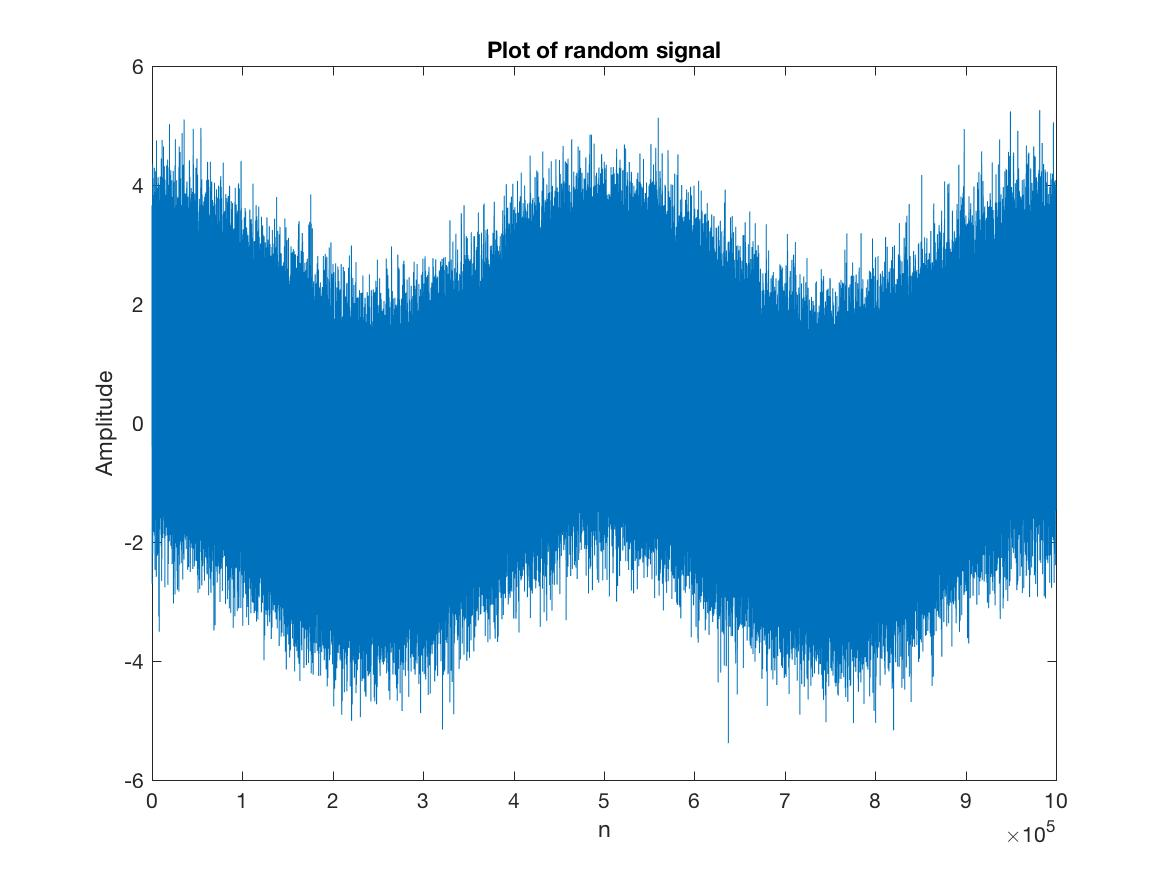
\includegraphics[width=4in]{Q3a.jpg}
\caption{random signal $x[n]$}
\label{fig:graph}
\end{figure}

\item The plot of  signal $x[n]$ and $y_1[n]$ is shown in the plot below:
\begin{figure} [H]
\centering
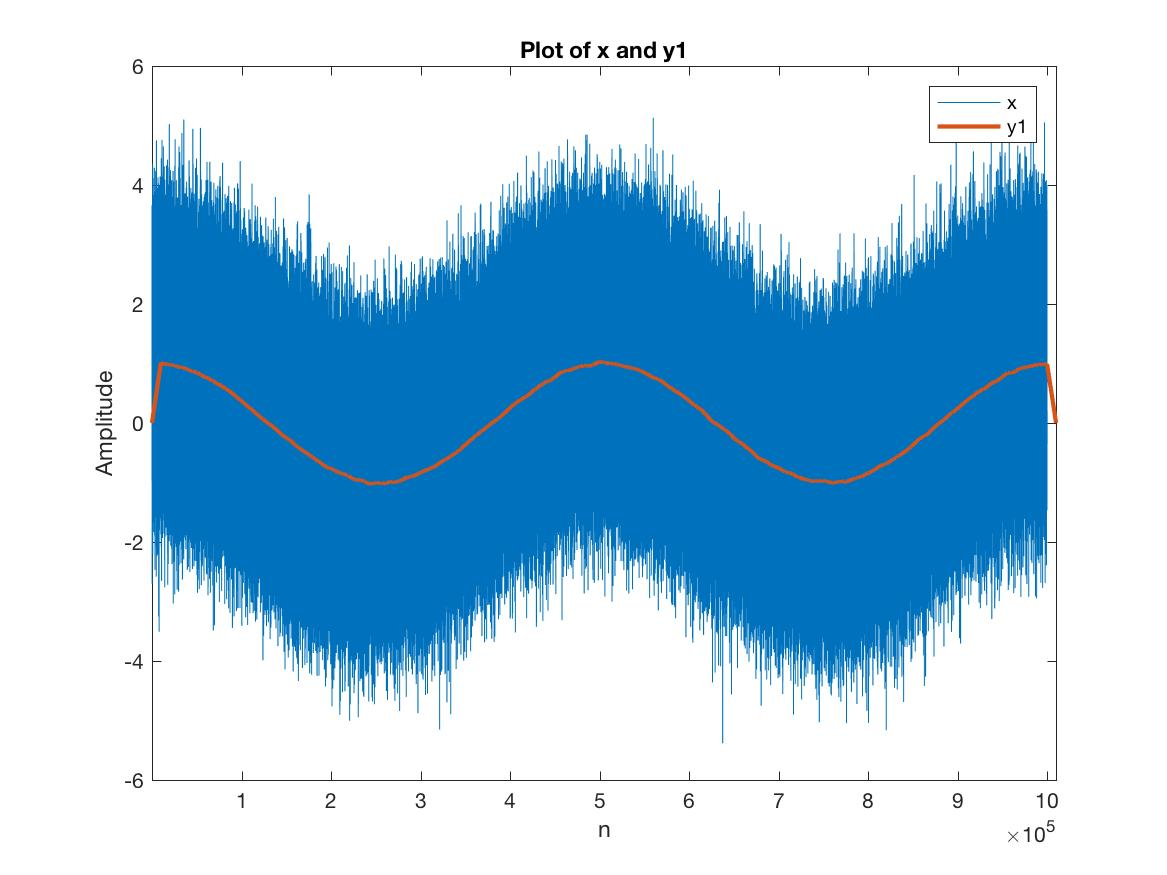
\includegraphics[width=4in]{Q3b.jpg}
\caption{Random signal $x[n]$ and the result of convolving it with an average filter}
\label{fig:graph}
\end{figure}

\item The overall shape of $y_1$ looks similar to x, but x has a much larger variance.

\item The plot of signal $x[n]$, $y_1[n]$ and $y_2[n]$ is shown below:
\begin{figure}[H]
\centering 
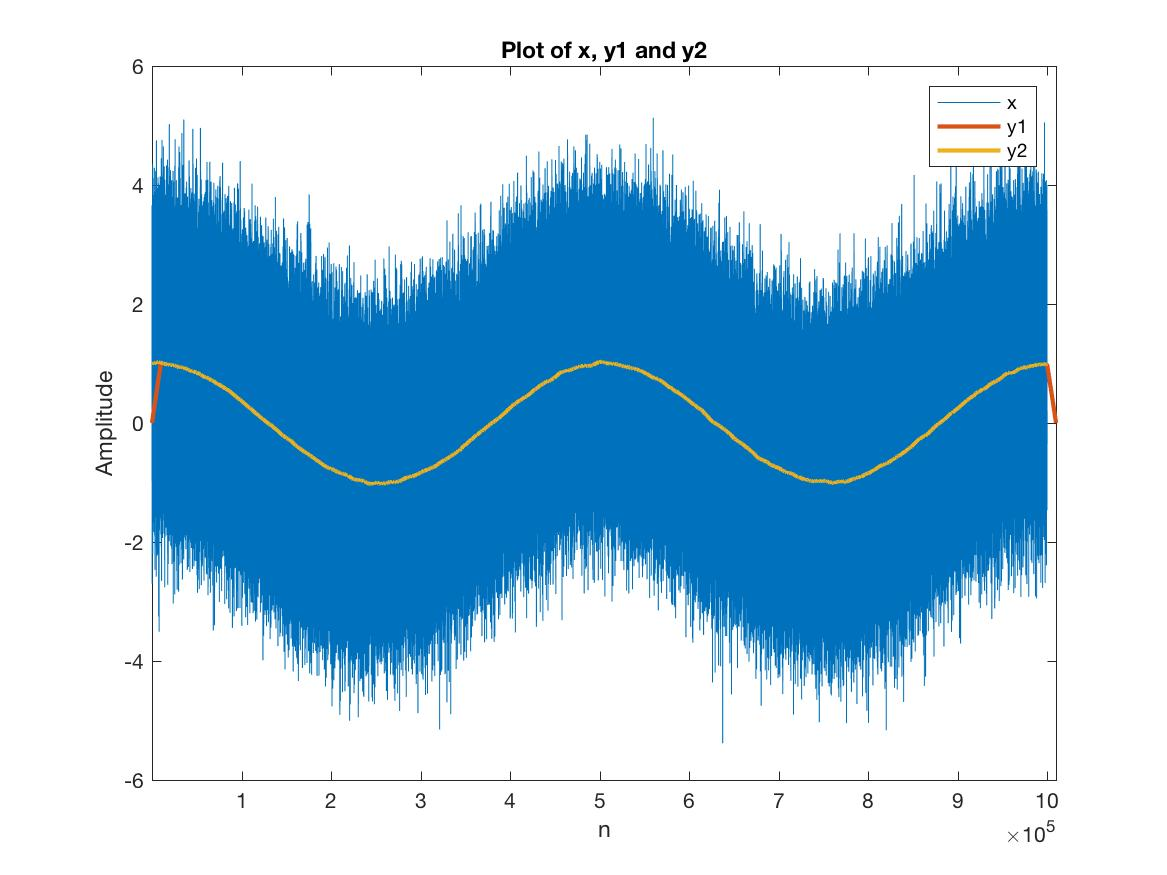
\includegraphics[width=4in]{Q3d.jpg}
\caption{Random signal $x[n]$, the result of convolving it with an average filter $y_1[n]$, the result using Fourier transform $y_2[n]$}
\end{figure}
\end{enumerate}

\Large\textbf{ Question \#4}:  \\
\normalsize
My UFID is 21959681. The name of matching music file is ``rudenko\_15.mp4".
\begin{figure}[H]
\centering
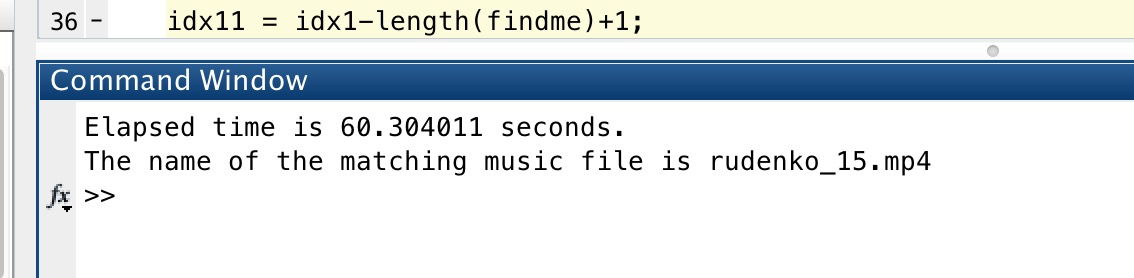
\includegraphics[width=4in]{Q4.jpg}
\end{figure}


\end{spacing}
\end{document}